\documentclass[twoside,openright,a4paper,12pt]{book}

\usepackage{mystyle}
\usepackage{glossaries}
\usepackage{float}

\makeatletter
\renewcommand\paragraph{\@startsection{paragraph}{4}{\z@}%
	{-2.5ex\@plus -1ex \@minus -.25ex}%
	{1.25ex \@plus .25ex}%
	{\normalfont\normalsize\bfseries}}
\makeatother
\setcounter{secnumdepth}{4} % how many sectioning levels to assign numbers to
<<<<<<< HEAD
\setcounter{tocdepth}{3}    % how many sectioning levels to show in ToC
=======
\setcounter{tocdepth}{2}    % how many sectioning levels to show in ToC
>>>>>>> master

\definecolor{pinegreen}{rgb}{0.0, 0.47, 0.44}
\newcommand{\ag}[1]{}

\loadglsentries{./chapters/defns}
\makeglossaries
\begin{document}

	\frontmatter%

	% La page de garde
	\thispagestyle{empty}

\begin{center}
	\noindent
	
\includegraphics[height=2.5cm]{./pics/logo_ufr.png}       
	
	\vfill\vfill
	
	{\large \textsc{Master de Science, Technologie, Santé \\mention Informatique\\spécialité Science et Ingénierie des Réseaux,\\de l'Internet et des Systèmes}}
	
	\bigskip\bigskip
	
	{\large Présenté par}
	
	\medskip
	
	% Identité de l'auteur
	{\large Constantin \textsc{Divriotis}}
	
	% Contact mail ou téléphone   
	{\small \url{constantin.divriotis@etu.unistra.fr}}
	
	\vfill\vfill
	
	% Titre du stage
	{\huge \sc
		\begin{center}
			\textit{Communications sécurisées\\intra-cloud et inter-cloud}
	\end{center}}
	
	\vfill\vfill
	
	{\large Encadré par}
	
	\medskip
	
	% Identité de l'encadrant
	{\large Andréas \textsc{Guillot}}
	
	% Contact mail ou téléphone
	{\small andres.guillot@unistra.fr}
	
	\bigskip
	
	{\large Au sein de}
	
	\medskip
	
	% Structure d'accueil
	{\large \textsc{Equipe réseaux - UFR Mathématiques et informatique de l'université de Strasbourg}}
	
	\vfill\vfill\vfill
	
	% Logo de votre structure d'accueil
	
\includegraphics[height=2.5cm]{./pics/icube.pdf}       
	
\end{center}

	% Page blanche au dos de la page de garde
	\newpage
	\pagestyle{empty}

	% La table des matières
	\renewcommand\contentsname{Table des matières}
    \begingroup
    \renewcommand{\cleardoublepage}{}
    \renewcommand{\clearpage}{}
	\tableofcontents
    \endgroup

	\mainmatter%

	\begingroup
\renewcommand{\cleardoublepage}{}
\renewcommand{\clearpage}{}
\chapter{Introduction}
\endgroup

L'objectif de ce sujet du Travail d'Étude et de Recherche est de modéliser un système de \textit{workflow} répondant à :
\begin{itemize}
	\item une authentification sécurisée de plusieurs acteurs d’un même système,
	\item une communication sécurisée entre plusieurs acteurs,
	\item une gestion de l’ordonnancement de plusieurs tâches entre elles.
\end{itemize}

Pour pouvoir répondre convenablement au sujet, nous nous limiterons à un cas d'étude particulier des systèmes de \textit{workflow} : le cloud informatique, appelé aussi \textit{cloud computing}. Nous nous intéresserons plus particulièrement à la communication sécurisée entre plusieurs acteurs au sein du \textit{cloud computing}.
\newline
La définition, fournie par l'institut national des standards et de la technologie (NIST) en 2011, permet de comprendre le but et les objectifs du cloud informatique (\cite{definition_cloud}) : « accès à distance via le réseau, à la demande et en libre-
service, à des ressources informatiques partagées
configurables ». Le \textit{cloud computing} se compose par plusieurs fonctionnalités
importantes telles que : il est accessible à distance n’importe où, et n'importe quand (mondialisation), c'est un service à la demande (Rapidité, facilité, flexibilité, scalabilité) et proposant une haute disponibilité du service (\textit{Service Level Agreement} (\gls{SLA})) et une sécurité des données (stockage sécurisé) et impliquant une démarche éco-responsable.
Le NIST présente également différents modèles de cloud.
Tout d'abord, il existe le cloud privé proposant une infrastructure exclusivement réservée à une entreprise ou une organisation.
Le cloud communautaire, lui, est une infrastructure réservée à une communauté d'organisations partageant des objectifs communs (politique de sécurité par exemple). Puis, le cloud public est une infrastructure appartenant à une entité et proposant des services payants accessible par le grand public. Enfin, il existe le cloud hybride, qui est une infrastructure composée de plusieurs types de cloud.
Dans ce document, les principales cibles d'attaques sont les clouds publics c'est pourquoi nous nous focaliserons dessus. Le nombre de données et de personnes plus élevés que sur les autres modèles de cloud ouvrent plus de possibilités aux \textit{\gls{Black Hats}}.

Les caractéristiques du cloud informatique ont créées une certaine popularité de cette nouvelle forme de stockage dans l'industrie et dans les académies, à tel point que même certaines infrastructures importantes et critiques (banque, NASA) soient tentées de migrer vers le cloud. L'enjeu et obstacle principal du cloud informatique à l'heure actuelle est la sécurité du cloud, qui empêche notamment son utilisation unanime \cite{security_cloud_issues}.

La sécurité du cloud implique des concepts tels que la sécurité des réseaux, du
matériel, mais également la sécurité de nouveaux concepts tels que la
virtualisation et de l'architecture \textit{multi-tenant}. En effet, les
solutions de sécurité actuelles proposent des solutions contre des menaces
provenant de l'extérieur afin de protéger le réseau intérieur, mais cette
approche n'est plus viable avec le cloud \cite{defcon17} \cite{defcon20}. En
effet, le système ne peut plus avoir confiance dans son réseau interne, car un
utilisateur malicieux peut être présent sur le réseau interne. Des nouvelles
attaques ont émergées suite à l'arrivé du cloud \cite{new_attack_cloud}. La sécurité dans le cloud fait alors appel à une série de politiques de sécurité et de technologies dans le but de protéger les données, informations, applications et infrastructures permettant d'assurer la sécurité du cloud en validant certains propriétés :
\begin{description}
	\item[Disponibilité :] les ressources du cloud sont toujours accessible aux utilisateurs.
	\item[Integrité :] la modification ou la suppression par des utilisateurs non autorisés est impossible et le cloud permet de vérifier que les données n'ont pas été altérées.
	\item[Confidentialité :] les données des utilisateurs sont secrètes et aucun autre utilisateur n'a de droit sur les données d'un autre utilisateur.
	\item[Contrôle :] gestion des ressources du cloud.
	\item[Authentification :] le cloud est capable de garantir que l'utilisateur est bien celui qu'il prétend lorsqu'un utilisateur agit sur les ressources du cloud et les utilise.
	\item[Non-répudation :] le cloud est capable de garantir les actions effectués sur des ressources par un utilisateur.
\end{description}

Dans un environnement cloud, le vecteur d'attaque principal est le réseau. Il apparaît crucial de sécuriser les communications internes et externes. Par conséquent, nous avons séparer les communications en deux catégories : les communications intra-cloud et inter-cloud.
Les communications intra-cloud impliquent de nouveaux concepts et ont générés
des nouveaux problèmes en terme de sécurité.
Le partage des communications sur une même
infrastructure et les réseaux virtuels sont des nouveaux challenges
dues aux nouveaux concepts du cloud. (\cite{security_cloud_survey}). Un routeur
virtuel est une instance d'un routeur physique, et plusieurs routeurs virtuels
peuvent s'exécuter en même temps sur un même routeur physique. On obtient alors
la possibilité de déployer plusieurs réseaux, que l'on appelle des réseaux
virtuels, sur un même réseau physique. Un réseau virtuel est un regroupement
d'un ensemble de routeurs virtuels compatibles. Les routeurs virtuels utilisent
les liaisons physiques pour s'interconnecter. Tous ces routeurs virtuels
doivent être isolés les uns des autres et cela implique une sécurité des
réseaux implacable à ce niveau. En effet, comme les \gls{VMs} (ou appelés
également machines virtuelles) partagent la même infrastructure réseau physique
et cela ouvre notamment la porte à des attaques de type cross-tenant
\cite{new_attack_cloud}. L'isolation des réseaux protège également contre des
attaques globales.
Les communications inter-cloud sont similaires
	aux communications sur Internet et donc, les différents problèmes de
	sécurité sont les mêmes.

Dans ce document, nous allons nous intéresser à la sécurité du cloud au niveau
du réseau au travers notamment des communications internes et externes du
cloud, car l'intégrité et la confidentialité des données peuvent être menacés à
chaque communication. Les solutions aujourd'hui pour assurer la sécurité du
cloud informatique passent notamment par l'utilisation de \gls{firewalls}, des \gls{IDS} et des \gls{IPS}. Sécuriser le réseau du cloud permet d'éviter de nombreuses attaques. 
Tout d'abord, le balayage de port qui se définit comme une attaque réseau visant à récupérer l'état des services réseaux d'une machine. L'attaque par déni de service, appelée \textit{Denial of Service} (DoS), est une attaque réseau pouvant cibler différents composants d'un système (processeur, mémoire) et visant à dégrader les performances du système. On parle maintenant d'attaque DDoS (\textit{Distributed Denial of Service}), car l'attaque est menée par plusieurs systèmes. L'attaque \textit{cross-tenant} exploite la mémoire cache L3, ce cache étant l’image miroir de la mémoire système et est partagé entre tous les utilisateurs sur un cloud \textit{multi-tenant}. Une personne malveillante va alors manipuler l’état de cette mémoire cache et attendre l’activité d’un utilisateur. En examinant les sections du cache modifiées, la personne malveillante peut trouver l’adresse mémoire contenant les données de l’utilisateur \cite{new_attack_cloud}. Le \textit{spoofing} se définit par l'usurpation d'identité visant à se faire passer pour quelqu'un d'autre dans le but de commettre différents actes malveillants. Enfin, on terminera par le \textit{sniffing} qui se caractérise par une écoute clandestine d'un réseau visant à lire et capturer les données qui transitent.

Nous allons tenter de répondre au problème suivant : comment obtenir un réseau
sécurisé tout en garantissant un niveau de performance élevé et une confiance
limitée à tous les niveaux. Nous allons tenter, dans ce rapport, de trouver les
meilleures solutions possibles actuelles et de comprendre quels éléments
peuvent être rajoutés à cette configuration pour obtenir une configuration
idéale. Le but de ce document sera donc de créer une solution cohérente qui
inclut le maximum de besoins et d’exigences en sécurité dans l’environnement cloud, mais cette solution doit être en balance entre les enjeux de sécurité et les enjeux de performance et de disponibilité du cloud. Ce document se base principalement sur l'étude effectuée par Mazhar et al. \cite{security_cloud_survey}.

Nous allons poser différentes hypothèses liées à notre problématique auxquels nous allons chercher à répondre par des solutions concrètes :
\begin{description}
	 \item[Hypothèse de stockage :] aucune confiance, les données du cloud ne
         doivent jamais être rendues publiques ou être victime d'une violation
         de données.
	 \item[Hypothèse d'utilisateur :] confiance limité avec l'utilisateur, ce dernier peut provoquer des fuites de données.
	 \item[Hypothèse du réseau :] aucune confiance au réseau, les données ne doivent pas être visibles et lues par une personne malveillante écoutant le réseau.
\end{description}

La figure \ref{fig:roadmap} décrit les différents challenges au niveau de la sécurité et souligne les parties, en rouge, dont nous allons nous préoccuper principalement. Ce modèle fait écho aux hypothèses que nous avons posé et nous allons nous baser notamment sur l'étude effectuée \cite{security_cloud_survey}) qui découpe la sécurité du cloud en plusieurs sections distinctes et propose différentes solutions pertinentes.

\begin{figure}[h]
\centering
\begin{tikzpicture}[y=-1cm, scale=0.9, x=-1cm]
\begin{scope}[every node/.style={ellipse, draw}]
	\node (A) at (-0.5,1) {Sécurité du Cloud};
	\node (B) at (-4,2) {Communication};
	\node (C) at (3,2) {Architecture};
	\node (HY) at (-0.5, 2.5) {Matériel};
	\node (FA) at (-9,1) {Famille};
\end{scope}

\begin{scope}[every node/.style={ellipse, draw, align=center}]
	\node (H) at (7,4) {Virtualisation};
	\node (J) at (2.4,4) {Stockage};
\end{scope}
\begin{scope}[every node/.style={ellipse, draw=red, align=center, line width=3pt}]
	\node (F) at (-6.85,4) {Externe};
	\node (G) at (-3.85,4) {Interne};
\end{scope}
\begin{scope}[every node/.style={fill=white,circle,bottom},
              every path/.style={draw=black, thick}]
	\path [->] (A) -- (B);
	\path [->] (A) -- (C);
	\path [->] (A) -- (HY);
	\path [->] (C) -- (H);
	\path [->] (C) -- (J);
	\path [->] (HY) -- (J);
	\path [->] (B) -- (G);
	\path [->] (B) -- (F);

\end{scope}
\begin{scope}[every node/.style={draw=red, rounded rectangle, align=center,
    line width=3pt}]
		\node (TR) at (-4,6) {Logiciel};
		\node (LI) at (3,6) {Réseau};
		\node (TI) at (-0.5,6) {Hardware};
\end{scope}
\begin{scope}[every node/.style={draw, rounded rectangle, align=center}]
		\node (FA) at (-9,3) {Méchanismes};
\end{scope}
\begin{scope}[every node/.style={fill=white,circle,bottom},
								every path/.style={draw=black, thick}]
		\path [->] (H) -- (TR);
		\path [->] (H) -- (LI);
		\path [->] (H) -- (TI);
		\path [->] (J) -- (TR);
		\path [->] (J) -- (LI);
		\path [->] (J) -- (TI);
\end{scope}
\begin{scope}[every node/.style={fill=white,circle,bottom},
every path/.style={draw=red, densely dotted, line width=3pt}]
	\path [->] (G) -- (TR);
	\path [->] (G) -- (LI);
	\path [->] (G) -- (TI);
\end{scope}
\begin{scope}[every node/.style={draw=red, rectangle, align=center, line width=3pt}]
	\node (ZA) at (3,8) {IDS, IPS};
	\node (ZB) at (-4,8) {Firewall};
	\node (ZC) at (-.5,8) {Politique de\\sécurité};
\end{scope}
\begin{scope}[every node/.style={draw, rectangle, align=center}]
	\node (ZZ) at (-9,5) {Outils};
\end{scope}
\begin{scope}[every node/.style={fill=white,circle,bottom},
	every path/.style={draw=red, densely dotted, line width=3pt}]
	\path [->] (LI) -- (ZA);
	\path [->] (TR) -- (ZB);
	\path [->] (TI) -- (ZC);
	\end{scope}
\end{tikzpicture}
\caption{Challenges de la sécurité du cloud}
  \label{fig:roadmap}
\end{figure}

Ce document est organisé de la manière suivante : le chapitre 2 contient un
état de l'art de la sécurité dans le cloud informatique structuré autour de trois
axes : la stockage~\ref{sec:sto}, la virtualisation~\ref{sec:vir}, et l'authentification et le contrôle
d'accès~\ref{sec:auth}.
Le chapitre 3 analysera différentes méthodes de la littérature pour les
communications réseaux dans le cloud, avec une séparation entre les
communications inter-cloud~\ref{sec:inter_cloud} dans un premier temps, puis les communications
intra-cloud~\ref{sec:intra_cloud}.

	\begingroup
\renewcommand{\cleardoublepage}{}
\renewcommand{\clearpage}{}
\chapter{État de l'art}
\endgroup

Ce chapitre va s'intéresser en premier lieu à l'hypothèse du stockage sécurisé dans un
environnement cloud. Puis, le chapitre va s'intéresser à de potentielles solutions des challenges posés au niveau de la virtualisation en terme de sécurité. Enfin, on discutera d'une solution garantissant une authentification sécurisée de plusieurs acteurs d’un même système

\section{Stockage}\label{sec:sto}

Le stockage est l'une des trois hypothèses posées dans l'introduction. Pour
pouvoir nous focaliser sur les communications dans un environnement cloud, il
est capital d'établir un schéma avec un stockage sécurisé. Le stockage est un
élément central dans l'environnement cloud. Le cloud n’offre pas tous les
droits à l’utilisateur sur les données. En effet, un utilisateur n'a qu'un
droit de contrôle sur la VM sur laquelle dont il est l'utilisateur. Les
fournisseurs de service de cloud (appelé CSP pour \textit{Cloud Service Provider}), eux, ont le rôle de gérer les données
et les serveurs. Mais, ce niveau de contrôle doit être maîtrisé et vérifié, car
l'environnement cloud (architecture \textit{multi-tenant} et virtualisation) a généré de nouvelles menaces. Le stockage doit faire face différentes menaces : une confidentialité et une intégrité des données non maîtrisées, une vulnérabilité sur la récupération des données (données d'un utilisateur ayant eu la même image précédemment), un mauvais nettoyage des supports (changement de disque nécessaire ou données stockées inutilisées), un \textit{backup} des données non sécurisé, des vulnérabilités via les applications Web (\cite{web_security}) ou encore une authentification et un contrôle d'accès insuffisamment efficace.

Dans cet optique, nous avons suivi les principales recommandations du CSA
(\textit{Cloud Security Alliance}) en terme de gestion des clés et de stockage des données (\cite{security_guidelines}) :
Premièrement, la gestion des clés doit être effectuée par les organisations/utilisateurs eux-mêmes ou bien par un service cryptographique de confiance avec un service crédible et neutre. Deuxièmement, les meilleurs pratiques pour la gestion des clés et de chiffrement provenant de source fiable doivent être utilisées. Troisièmement, il est recommandé d'utiliser une technologie standardisée dans la mesure du possible. Quatrièmement, la portée d'une clé ne doit pas dépasser un utilisateur ou un groupe d'utilisateur. Enfin, l'utilisation d'algorithmes standards est recommandée et les algorithmes de chiffrement propriétaires sont déconseillés.

Sur la base de l'étude \cite{security_cloud_survey}, il en ressort plusieurs solutions. Nous avons décidé d'en retenir deux dans le but d'offrir des approches différentes selon le stockage souhaité. Ces deux solutions ont été choisies, car elles mettent en place les recommandations de sécurité du CSA \cite{security_guidelines}. De plus, les solutions sont présentées dans le papier Mazhar et al \cite{security_cloud_survey} et ont l'avantage d'être des solutions récentes pour sécuriser le stockage dans le cloud : FADE (\cite{fade}), SecCloud (\cite{secCloud}).

\subsection{FADE}

FADE (\textit{File Assured Deletion}) est un protocole permettant une gestion de clés cryptographiques et utilisant des techniques de cryptographie symétriques et asymétriques. Ce protocole garantit une confidentialité et une intégrité des données dans un environnement cloud en fonctionnant avec des groupes de gestion de clés (KM pour \textit{key manager}) agissant comme un \gls{TPA} (\textit{Trusted Party Third}) et générant des clés publiques/privées.
Différents cryptages sur les mêmes données permettent de sécuriser ces dernières et d'effectuer un contrôle d'accès implicite des données. Le fonctionnement du protocole est décrit sur la figure \ref{label-image1} : pour encrypter un fichier F de l'utilisateur, une clé de donnée aléatoire K est utilisée. Ce fichier F, encrypté par K, sera encrypté par une clé symétrique S. Enfin, la paire de clé générée par KM encrypte S. Un ficher de politique d'accès P permet de vérifier qui peut accéder au fichier. 
\newline
Pour télécharger un fichier stocké cloud, un utilisateur doit effectuer une requête en envoyant P auprès du KM afin qu'il lui délivre une paire de clé publique/privée. La clé publique sera transmise à l'utilisateur qui encryptera le fichier F en encryptant F avec K et K avec S. Enfin, la clé publique, délivrée par KM, encryptera S. Le fichier F est stockée dans le cloud avec un haut niveau de cryptage et avec le fichier P. Pour décrypter un fichier stocké dans le cloud, il est nécessaire que l'utilisateur envoie S à KM afin de décrypter le fichier, puis décrypter F. 
\newline
Enfin, un écrasement sécurisé des clés cryptographiques et d'un fichier de politique (politique vis-à-vis des accès au fichier stocké sur le cloud par un utilisateur) permet de rendre les données inaccessibles et donc assurément supprimées.
\newline 
Une solution retenue pour le stockage dans le cloud est FADE, car elle permet un contrôle d'accès et une suppression définitive des données, tout en proposant un scalabilité élevé, un cryptage des données avec l'aide d'un TPA et garantit l'intégrité et la confidentialité des données.

\begin{figure}[hb]
	\center
	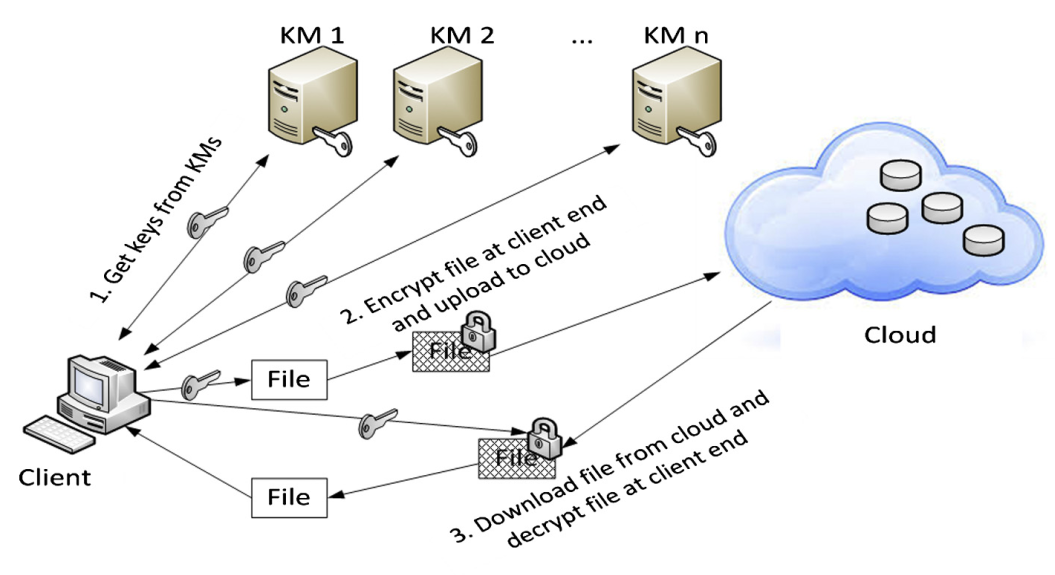
\includegraphics[height=7.5cm]{./pics/schema_fade.png}
	\caption{Fonctionnement du protocole FADE [\cite{security_cloud_survey}]}
	\label{label-image1}
\end{figure}

\subsection{SecCloud}
SecCloud est un protocole cherchant à protéger les données stockées par un utilisateur, mais également les calculs effectués sur ces données. Le protocole se base sur l'utilisation d'une cryptographie à base de couplage pour permettre de générer des clés pour les utilisateurs, le CSP et un TPA. Un utilisateur peut alors stocker ses données dans l'espace de stockage fourni par un CSP et ces données sont signées par un TPA. Les données sont alors envoyées au cloud avec la signature du TPA et encryptées avec une clé de session. Le cloud va alors décrypté ces données, vérifié la signature du TPA et stocké les données dans les partitions désignées dans le but d'empêcher toute violation des données. 
L'algorithme Merkle Hash Tree, reconstruit par le TPA, permet de vérifier les calculs effectués sur les données. Le TPA a une place importante, car il a le devoir de vérifier l’accessibilité et l’intégrité des données sur requête du client.
\newline
SecCloud est une solution pertinente pour le stockage dans le cloud. L'utilisation d'un TPA, la vérification de signature et l'utilisation d'une cryptographie à base de couplage pour crypter les données sont des fonctionnalités alléchantes de cette solution. Elle assure la confidentialité et l'intégrité des données via ces fonctionnalités.

\section{Virtualisation}\label{sec:vir}

La virtualisation permet l’utilisation des mêmes ressources physiques pour
plusieurs utilisateurs. Une VM est instanciée pour chaque utilisateur et permet
alors à l’utilisateur d’avoir une machine complète et opérationnelle. Plusieurs machines virtuelles peuvent être sur les mêmes ressources physiques et créer un environnement multi-tenant.
Tout comme le stockage, la virtualisation soulève de nouveaux défis, car toutes
les ressources sont virtualisées (serveurs, stockage, équipements de réseau, etc.). En particulier, la connexion aux serveurs dans le cloud doit s'effectuer par le biais d'un réseau virtuel mis en place dans ce but et où les routeurs virtuels se déplacent en fonction des emplacements des ressources du CSP. Aujourd'hui, selon le type de menace, on peut recenser des solutions différentes. Dans cette partie, nous dresserons des tableaux comparatifs proposant des solutions adéquates à chaque problème de virtualisation.

\subsection{Migration}
La migration d'une VM est une opération courante effectuée dans le cloud afin d'équilibrer les charges au sein du cloud, remplacer des VMs tombées dû à des pannes physiques, économiser de l'énergie ou encore effectuer des mises à jour matérielles ou logicielles. 
La relocalisation d'une VM sur une autre machine physique sans éteindre la VM ouvre la porte à des problèmes d'intégrité et de confidentialité des données, car les données de la VM sont exposées au réseau. De plus, la migration elle-même est sujet aux attaques, comme une relocalisation d'une VM sur un serveur malveillant dans le but de prendre le contrôle total de la VM. La migration est une opération délicate qui nécessite une sécurité accrue. Le tableau comparatif \ref{label-image12} présente diverses solutions permettant de migrer une VM. De ce tableau, on peut retenir la solution appelée \textit{Framework for secure live VM migration} qui permet un cryptage des données lors de la migration, mais également un contrôle d'accès basé sur les rôles (\gls{RBAC}). Malgré une scalabilité moyenne, les apports supplémentaires de cette solution nous amènent à la plébisciter. En effet, elle apporte une sécurité contre les migrations inutiles, mais également contre les attaques \textit{\gls{VM hopping}} (attaque appelée également \textit{VM jumping}).

\begin{figure}[h]
	\center
	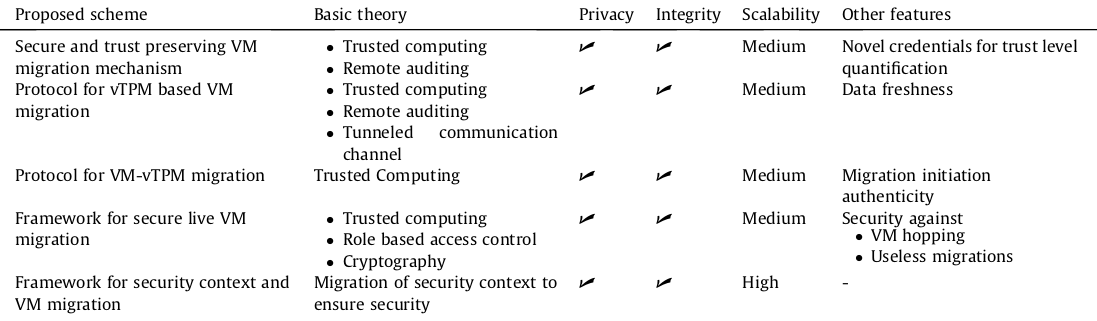
\includegraphics[width=15.5cm]{./pics/VM_migration_tableau.png}
	\caption{Comparaison de diverses solutions permettant une migration de VM sécurisée [\cite{security_cloud_survey}]}
	\label{label-image12}
\end{figure}

\subsection{Partage d'image}
Les images de VM permettent d'initialiser une VM. Pour ne pas corrompre une VM, elle doit être parfaitement intègre et sécurisée. Une fois en place dans le cloud, une VM infectée est capable de gérer son trafic entrant/sortant et peut endommager les données d'autres utilisateurs et créer des problèmes d'intégrité et de confidentialité.
La plupart du temps, les images des VMs sont utilisées par divers utilisateurs et certains utilisateurs malicieux seront tentés d'infecter certaines images en injectant un \textit{malware}. Autre possibilité, un utilisateur malicieux va chercher une faille et un point d'attaque dans le code public des images et si il est capable d'en trouver une, mettre en place une attaque contre ce type d'images. Le tableau comparatif \ref{label-image12} présente diverses solutions garantissant l'utilisation d'images sécurisées de VM. Ce tableau comparatif révèle que la solution \textit{EVDIC} est la plus adéquate. C'est la seule solution permettant une intégrité et une confidentialité des données. En terme de sécurité, il est préférable de protéger les données et de les préserver. On observe que les autres solutions apportent différentes fonctionnalités, mais dans le cadre d'un cloud public, la solution \textit{EVDIC} paraît la plus apte.

\begin{figure}[h]
	\center
	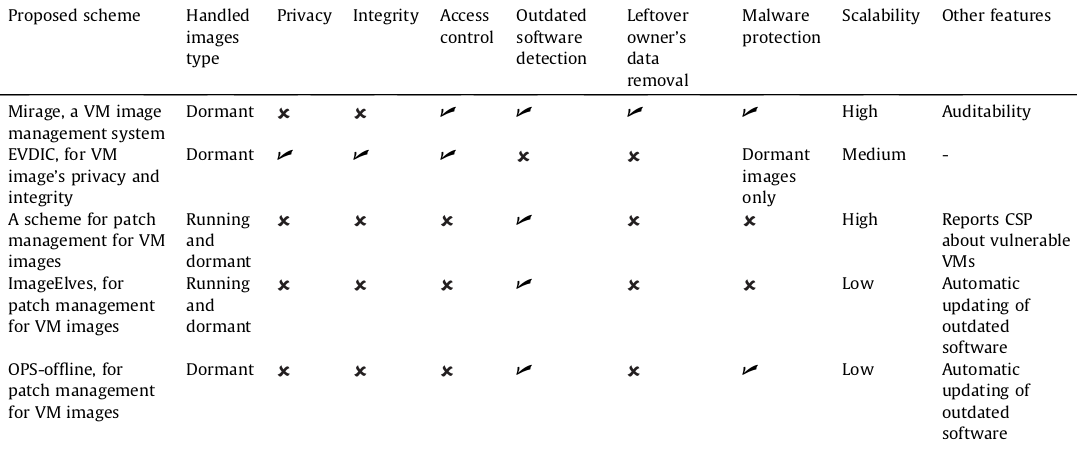
\includegraphics[width=15.5cm]{./pics/securing_VM_images_tableau.png}
	\caption{Comparaison de diverses solutions offrant des images de VM sécurisée [\cite{security_cloud_survey}]}
	\label{label-image13}
\end{figure}

\subsection{Exécution}
Lors de l'exécution d'une VM, cette dernière doit pouvoir offrir des garanties sur la sécurité de son environnement. Premièrement, l'isolation des VMs les unes des autres sur le même matériel (ou \textit{hardware}) physique est obligatoire, car elles sont sujet à des attaques \textit{cross-tenant} ou encore à l'apparition de brèches de données.
Durant l'exécution, des actions sont également sensibles à des attaques. Par exemple, des \textit{rollback} sont possibles sur une VM, mais ils peuvent poser des problèmes de sécurité : des autorisations données à certains utilisateurs non autorisés avant \textit{rollback} ou une modification de la configuration sont des exemples de problèmes de sécurité générés par des \textit{rollback}.
Le tableau comparatif \ref{label-image14} présente diverses solutions permettant de sécuriser l'exécution d'une VM.
Dans la continuité de nos propos, la solution \textit{HyperCoffer} est la plus adaptée à sécuriser l'exécution d'une VM. La séparation de la sécurité et du management des VMs couplée au cryptage des données assure une sécurité satisfaisante pour l'exécution d'une VM. Ce cryptage doit rester interne à la VM, car les données échangées dans le réseau virtuel doivent être en claires. Nous reviendrons sur ce point dans la section~\ref{sec:intra_cloud}. Enfin, en plus de fournir une haute scalabilité, elle permet d'effectuer des \textit{rollbacks} sécurisés.

\begin{figure}[h]
	\center
	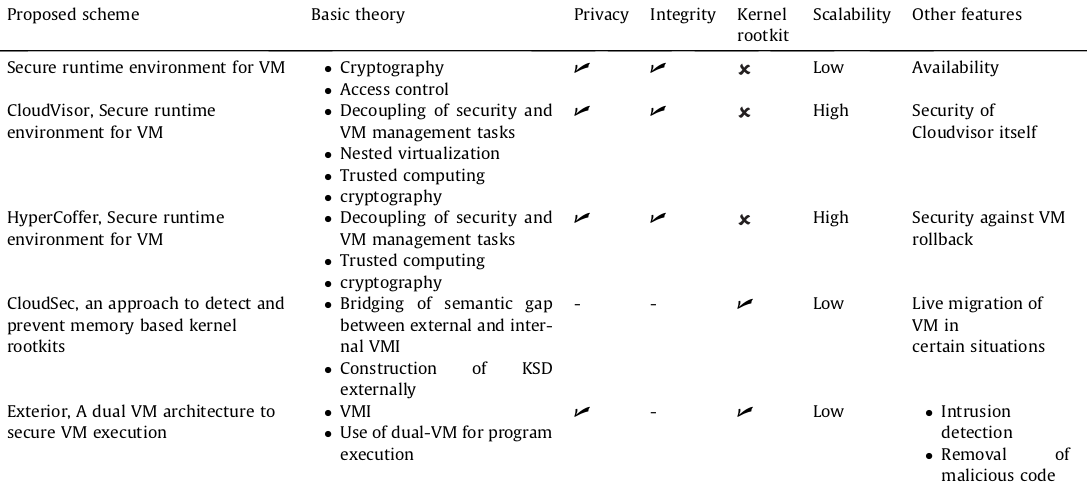
\includegraphics[width=15.5cm]{./pics/security_execution_VM_tableau.png}
	\caption{Comparaison de diverses solutions garantissant une exécution sécurisée d'une VM [\cite{security_cloud_survey}]}
	\label{label-image14}
\end{figure}

\subsection{Sécurité de l'hyperviseur}
Si l'\gls{hyperviseur}, appelé aussi \textit{Virtual Machine Monitor} (ou VMM) est compromise, toutes les VMs contrôlées par la VMM sont alors sous le contrôle d'une personne malveillante. En effet, une VMM tourne en mode privilégié. Si une VMM est compromise, un utilisateur malveillant est capable de s'attribuer des droits non autorisés. C'est pourquoi, notamment, les données des VMs transitant par la VMM sont en position critique posant des problèmes de confidentialité et d'intégrité. Le tableau comparatif \ref{label-image15} présente diverses solutions garantissant la sécurité de l'hyperviseur. Pour ce dernier tableau comparatif, on retiendra \textit{DeHype}. La protection des VMs est assurée. Cette solution sépare également la VMM et le système d'exploitation donnant lieu à un risque d'attaque amoindri provenant du système d'exploitation. Enfin, la réduction des droits privilégiés freine fortement les actions possibles si la VMM est sous le contrôle d'une personne malveillante. 

\begin{figure}[h]
	\center
	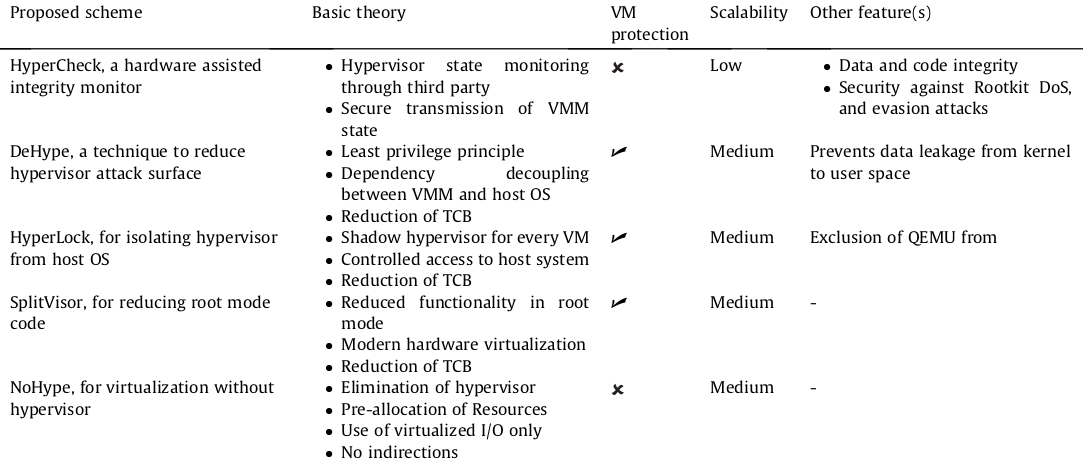
\includegraphics[width=15.5cm]{./pics/VMM_solutions_tableau.png}
	\caption{Comparaison de diverses solutions garantissant la sécurité de l'hyperviseur [\cite{security_cloud_survey}]}
	\label{label-image15}
\end{figure}

\section{Authentification et contrôle d'accès}\label{sec:auth}

Comme précédemment, le CSA (\cite{security_guidelines}) recommande certaines mesures de sécurité. Tout d'abord, l'utilisation de standards libre (OAuth, SAML \cite{security_guidelines}) est recommandée. Deuxièmement, les sources des attributs doivent être aussi proche possible de la \textit{master} source et les attributs doivent être validés par le \textit{master} ou équivalent. Troisièmement, les caractéristiques des entités doivent avoir un niveau de confiance identifié. Quatrièmement, une confiance bi-directionnelle est souhaitée entre deux entités afin d'avoir une relation et des transactions sécurisées. Enfin, les services doivent avoir la capacité d'exporter/importer avec des standards (\gls{XACML} \cite{xacml} \cite{security_guidelines}). 
\newline
La solution retenue pour cette gestion d'identité et ce contrôle d'accès est \textit{Hierarchical Attribute-Set-Based Encryption} (HASBE)\cite{hasbe}. Tout d'abord, elle a été retenue, car elle respecte les recommandations proposées par le CSA. De plus, dans l'étude effectuée \cite{security_cloud_survey}, un tableau comparatif des solutions de gestion d'identité et de contrôle d'accès permet de constater que c'est HASBE qui offre le plus de sécurité tout en offrant une scalabilité performante.
\newline
Pour introduire HASBE, il faut évoquer \textit{Attribute Based Encryption} (ABE) \cite{asb} qui a été utilisé pour fournir un contrôle d'accès dans un environnement cloud. Les messages encryptés sont associés aux attributs des utilisateurs. Ainsi, pour décrypter un message, il est nécessaire que l'utilisateur possède cet attribut. Puis, une extension de ABE, appelée \textit{Attribute Set Based Encryption} (ASBE) \cite{asbe} a introduit un arrangement récursif des attributs en les séparant par catégories permettant à l'utilisateur de pouvoir appliquer des contraintes dynamiques sur la manière dont les attributs remplissent la politique de contrôle d'accès. Enfin, HASBE, étant une extension de ASBE, pose une structure hiérarchique des utilisateurs en introduisant des autorités de confiance et des autorités de domaine. La figure \ref{label-image2} démontre le fonctionnement de HASBE. L'autorité de confiance administre les autorités de domaine qui gèrent à leur tour des autorités de domaine au niveau suivant ou des utilisateurs du domaine. L'autorité de confiance génère et délivre les paramètres systèmes (permettant de créer des groupes notamment) et la clé racine aux autorités de domaine. Les clés sont générées à l'aide de groupes multiplicatifs bilinéaires et les clés asymétriques sont délivrées aux utilisateurs par les autorités de domaine. Ces clés asymétriques sont des \textit{Tree structure based key} c'est-à-dire des structures d'arborescentes hiérarchiques ou chaque élément étant un attribut ou un ensemble d'attribut. Le contrôle d'accès est défini comme une arborescence hiérarchique et il est assuré uniquement pour les données dans le cloud. Enfin, les données sont cryptées avec une clé de cryptage, clé protégée avec le HASBE utilisant la structure d'accès des clés qui spécifie les politiques et attributs de contrôle d'accès. L'accès au déchiffrement est possible pour les utilisateurs possédant les attributs et les accès dans la structure des clés d'accès.
HASBE a été retenue pour couvrir la sécurité de l'authentification et du contrôle d'accès. HASBE fournit un chiffrement par attributs, un accès aux données contrôlée et une mise en place d'une hiérarchie de confiance. Supportant une haute scalabilité, HASBE se voit être la meilleure solution pour répondre à l'hypothèse d'authentification sécurisée de plusieurs acteurs d'un même système.

\begin{figure}[hb]
	\center
	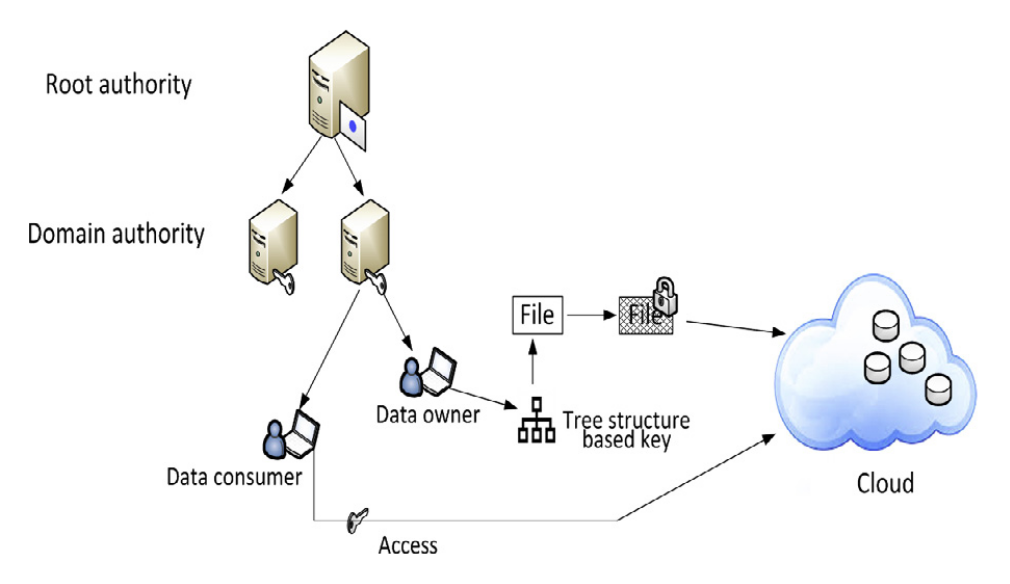
\includegraphics[height=7.5cm]{./pics/hasbe.png}
	\caption{Fonctionnement de HASBE[\cite{security_cloud_survey}]}
	\label{label-image2}
\end{figure}

	\begingroup
\renewcommand{\cleardoublepage}{}
\renewcommand{\clearpage}{}
\chapter{Communications cloud}
\endgroup

Pour commencer, il est primordial de rappeler que la plupart du temps, les services du cloud sont accessibles par les utilisateurs via Internet \cite{internet_cloud}. Le protocole IP et ses mécanismes sont utilisés pour permettre la communication entre l'utilisateur et le cloud \cite{use_ip_cloud} afin de délivrer les services du cloud et assurer l'échange de données.

\section{Communications inter-cloud}\label{sec:inter_cloud}

Les communications inter-cloud sont similaires aux autres communications sur Internet et posent les mêmes problématiques en terme de sécurité. Ces problèmes de sécurité interviennent au plus haut de la couche à la plus basse de la pile \gls{TCP/IP} et chacune ajoute de l'information dans les paquets envoyés. Heureusement, des solutions existent et la sécurité est présente dans plusieurs couches du modèle TCP/IP. Toutefois, il n'est pas toujours nécessaire de crypter et sécuriser chaque couche.

\begin{description}
	\item[Couche application :] utilise des mécanismes de sécurité pour une application donnée, séparés des autres couches. \textit{Pretty Good Privacy} (PGP) \cite{pgp} est un exemple d'utilisation sur la couche application. L'envoi de courrier électronique sécurisés est possible grâce aux fonctionnalités de PGP : chiffrer des textes et les signer.  
	\item[Couche transport :] des contrôles de sécurité permettent de protéger les données en transit entre deux hôtes distants. \textit{Transport Layer Security} \cite{tls} et \textit{Secure Sockets Layer} \cite{ssl} sont des protocoles cryptographiques permettent de sécuriser les échanges sur Internet via la couche transport. Ils permettent l'authentification de l'hôte distant et la confidentialité et l'intégrité des données échangées. Des modifications peuvent être nécessaire à certaines applications pour utiliser ces protocoles. 
	\item[Couche réseau :] toutes les communications entre deux hôtes ou avec le réseau peuvent être protégées avec cette couche sans modification spécifique. IPSec \cite{ip_security} est un ensemble de protocoles utilisant des algorithmes garantissant des échanges sécurisés en authentifiant et chiffrant chaque paquet entre deux hôtes distants.
\end{description}

La sécurité au niveau de la couche réseau est la solution la plus souvent utilisée pour protéger l'ensemble des applications et les informations IP. IPSec est utilisé majoritairement pour fournir un \textit{Virtual Private Networking} (VPN) \cite{ipsec_vpn}, plus précisément un VPN site-à-site. Un VPN est un réseau privé virtuel, construit sur un réseau physique existant et fournissant un lien direct entre deux hôtes distants et offrant un échange de données sécurisé. En effet, en isolant le trafic entre les deux hôtes distants, un VPN facilite la sécurité de la communication  sur des réseaux publics. Un VPN site-à-site permet d'établir plusieurs connexions sécurisés avec plusieurs hôtes situés à différentes locations entre eux afin de former un groupe d'utilisateurs fermés, appelé \textit{Closed User Group} (CUG). Aujourd'hui, via le service IPSecVPN, les connexions inter-cloud permettent d'offrir des garanties de sécurité satisfaisantes. Cependant, le nombre d'utilisateurs se connectant aux CSP va augmenter considérablement et vont, sans doute, utiliser plusieurs services de cloud différents. Ainsi, le nombre de réseaux clouds connectés via IPSec VPN va augmenter considérablement également. Il est nécessaire donc de proposer une solution durable et performante basé sur IPSecVPN.

\begin{figure}[h]
	\center
	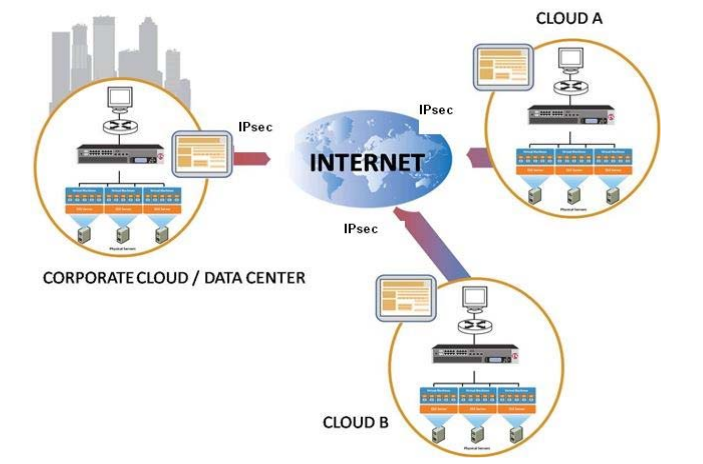
\includegraphics[height=5.5cm]{./pics/inter_cloud_archi_general.png}
	\caption{Architecture général des communications inter-cloud \cite{archi_inter}}
	\label{label-image3}
\end{figure}

Dayananda M. S. et Ashwin K. proposent une architecture pour les communications inter-cloud utilisant IPSecVPN \cite{archi_inter}. Il existe deux types d'architecture IPSecVPN principales : \textit{Full Mesh} et \textit{Hub-and-Spoke}. L'architecture \textit{Full Mesh} se caractérise par une connections de tous les réseaux entre eux et les réseaux vont communiqués en utilisant IPSec. L'architecture \textit{Hub-and-Spoke} est le modèle le plus utilisé avec un \textit{hub} placé entre tous les réseaux et les connectant. Un seul lien IPSec est nécessaire, c'est le lien entre le réseau et le \textit{hub}.
Les deux architectures présentent chacune des problèmes de performance, par exemple, lorsque le nombre de CUG augmente ou encore lorsque le trafic entre les CUG augmente. Pour résoudre le problème de performance, il se base sur l'architecture textit{Hub-and-Spoke} afin de mettre en place un système de IPSecVPN qui créer dynamiquement les tunnels entre les différents clouds en fonction de la demande.
\newline
L'architecture proposée permet tout d'abord d'établir des connexions IPSec dynamiques via des accès VPN multi-points en combinant le chiffrement d'IPSec, des tunnels \textit{Generic Routing Encapsulation} (\gls{GRE}) et le protocole \textit{Next Hop Resolution} (\gls{NHRP}). Il est nécessaire que chaque routeur (autre que le \textit{Hub}) possède une interface point-à-point afin de pouvoir créer le tunnel vers le \textit{Hub}. On oblige alors tout le trafic entre les routeurs, appelé \textit{Spoke}, a transité par le \textit{Hub}. De plus, si un \textit{Spoke} transmet des données, le \textit{Hub} agit alors comme serveur NHRP afin de déterminer dynamiquement l'adresse de destination. Il est à noter que lorsque le \textit{Hub} agit comme serveur NHRP, il permet à GRE de configurer et déterminer les adresses de destination les plus courtes des autres pairs. Les deux routeurs, source et destination, vont alors lancer IPSec entre eux et ainsi créer dynamiquement un tunnel GRE point-à-point, mais également commencer les négociations des sessions IPSec directement sans configuration traditionnelle (gain de temps considérable). Ce tunnel sera automatiquement tombé après une certaine période d'activité. Ensuite, autre avantage de ce type de configuration est que les \textit{Spoke} peuvent utiliser une adresse IP dynamique, car NHRP permet de déterminer l'adresse IP de l'interface du \textit{Spoke} distant via le routeur \textit{Hub}. Enfin, dernier avantage, la configuration du \textit{Hub} est grandement simplifiée puisqu'elle n'a pas besoin de configurer les informations GRE ou IPSec des \textit{Spoke}, car elles sont apprises dynamiquement via NHRP. De plus, la configuration permet d'ajouter un nouveau \textit{Spoke} sans configuration supplémentaire, car ce dernier va s'enregistrer auprès du \textit{Hub} dynamiquement et les différentes informations du nouveau \textit{Spoke} seront propagées vers les autres pairs et inversement. Pour finir, l'architecture proposée, sur la figure \ref{label-image4}, apporte également une autre fonctionnalité : lorsqu'une nouvelle connexion IPSec/IKE est établie entre deux \textit{Spoke}, les règles de filtrage de \textit{Hub} ne sont pas appliqués entre eux. L'utilisation d'une extension du \textit{Traffic Selector} (TS) permet de placer les différents filtres dans la création de la session IPSec/IKE afin d'établir les règles de filtrage dans l'échange IPSec/IKE entre les deux \textit{Spoke}.

\begin{figure}[h]
	\center
	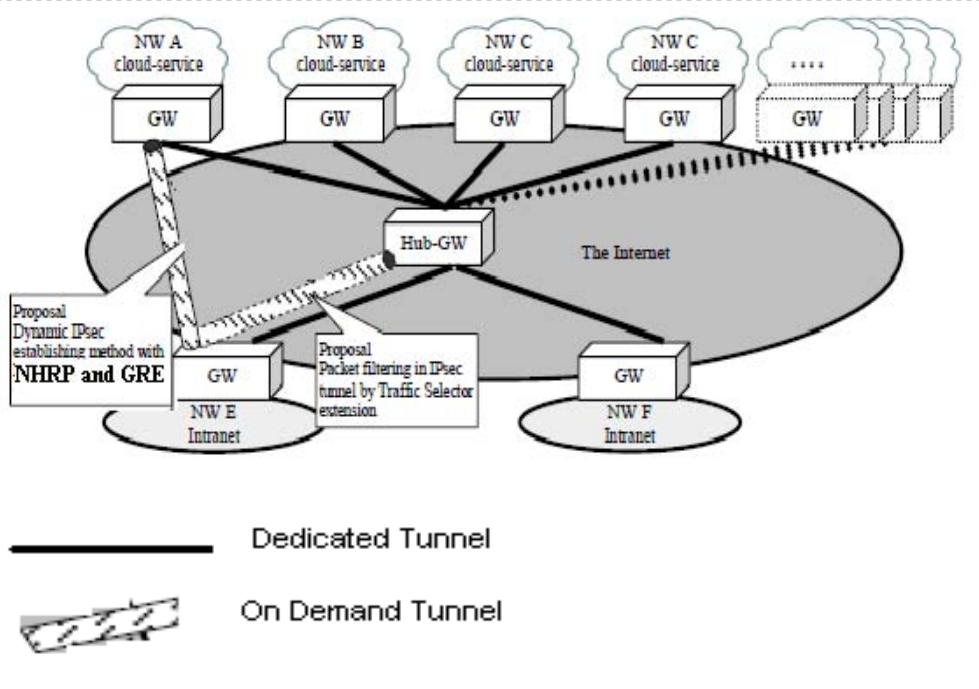
\includegraphics[height=5.5cm]{./pics/inter_cloud_architecture.png}
	\caption{Architecture proposé pour les communications inter-cloud \cite{archi_inter}}
	\label{label-image4}
\end{figure}

En conclusion, l'architecture proposé, appelé Dynamic Multipoint VPN, permet aux utilisateurs (ici, les fournisseurs de cloud) de mieux adapter les tunnels IPSecVPN en combinant le chiffrement d'IPSec, des tunnels GRE (\gls{GRE}) et le protocole NHRP. Les différents problèmes rencontrés dans les autres topologies IPSec VPN, Full-Mesh et Hub-and-Spoke, sont résolues avec les solutions proposées par cette architecture (voir \ref{label-image8}).

\begin{figure}[h]
	\center
	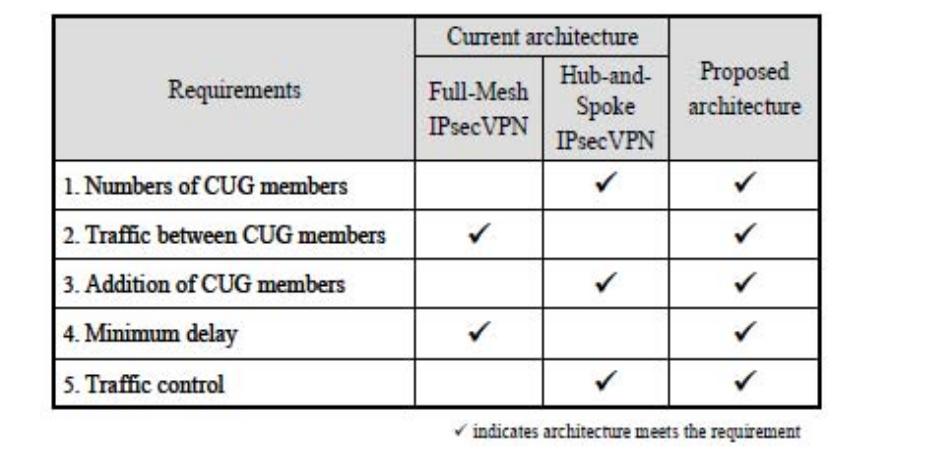
\includegraphics[height=5.5cm]{./pics/comparative_archi_inter_cloud.png}
	\caption{Comparaison des architectures IPSec VPN \cite{archi_inter}}
	\label{label-image8}
\end{figure}

Le cloud implique de nouveaux problèmes du à l'utilisation de l'architecture \textit{multi-tenant}. Une VM peut être corrompue et peut agir de manière malveillante. Un hôte interne du réseau est alors infecté et cible alors les machines du cloud. On parle alors d'une attaque interne impliquant les communications intra-cloud.
La deuxième partie du problème est donc de pouvoir sécuriser le cloud de possibles attaques internes. La démonstration de ce type d'attaque a été démontrée lors de la conférence
DefCon 18 par Bryan et Anderson (\cite{faiblesse_cloud}). Une attaque DDoS a été mise en place depuis le cloud EC2 d'Amazon et ils ciblaient une autre machine virtuelle, sur le même réseau.

\section{Communications intra-cloud}\label{sec:intra_cloud}

Aujourd'hui, les solutions actuelles, mises en place dans les cloud pour le sécuriser, utilisent des firewalls, des IDS et des IPS. Dans cette partie, nous allons tenter de proposer une solution performante en se basant sur le papier de Mazhar et al \cite{security_cloud_survey}. De plus, on ajoutera que le CSA (\cite{security_guidelines}) recommande l'utilisation de combinaisons de différents \gls{LAN} virtuels, d'IDS, d'IPS et d'un firewall afin de protéger les données en transit dans le cloud. 

\subsection{Solutions NIDS pour le cloud}

\subsubsection{SnortFlow}
\ag{Trop d'itemize}

\textit{SnortFlow} \cite{snortflow} est une solution proposée visant à améliorer les performances de \textit{Snort}. \textit{Snort} est un NIDS (Network IDS) orienté IDS/IPS : ce sont des solutions permettant de surveiller en temps réel un système et de détecter des activités suspectes violant la politique de sécurité du système. \textit{Snort} permet d'analyser le trafic en temps réel et enregistrer les paquets (log) au-dessus du protocole IP. Mais, les services proposées ne s'arrêtent pas là : 
recherche et correspondance de contenu, inhiber les \gls{prises d'empreintes} de la pile TCP/IP, dépassement de \textit{buffer}, scans, attaque CGI (Common Gateway Interface), sondes SMB (Server Message Block).
\textit{Snort} propose trois modes d'action du NIDS : le mode \textit{Sniffer} lit les paquets et les affiche, le mode \textit{Packet Logger} permet d'obtenir une log des paquets sur le disque et enfin, le mode \textit{Network Intrusion Detection System} qui gère le trafic et l'analyse avec les règles fixées par l'administrateur. Toutefois, le trafic ne doit pas être crypté, sinon le NIDS n'est plus capable de l'analyser.
Le fonctionnement de \textit{Snortflow} se base sur \textit{Snort} en ajoutant les fonctionnalités d'\textit{\gls{OpenFlow}}. \textit{OpenFlow} présente une nouvelle architecture pour fournir un environnement de réseau virtuel. L'idée sous-jacente est la séparation physique des plans de contrôle et de données. C'est la raison pour laquelle différents éléments exécutent la procédure de transfert de paquets (plan de données) et la procédure de contrôle de réseau (plan de contrôle). Le transfert est effectué grâce à une table de transfert partagée qui représente le plan de données, tandis que tous les plans de contrôle sont centralisées dans un nœud appelé contrôleur ou \textit{Controller}, faisant fonctionner les applications qui contrôlent le réseau virtuel. Ce contrôleur est un élément central du réseau. Il peut communiquer avec tous les nœuds pour configurer les tables de flux. Il travaille comme une interface entre les applications du réseau et les nœuds de transfert. Dans \textit{SnortFlow}, \textit{OpenFlow} est associé à \gls{POX}. Chaque plan de contrôle est composé d'un jeu d'application tournant sur POX. C'est la raison pour laquelle, dans \textit{OpenFlow}, un réseau virtuel est défini par son plan de contrôle, qui est un jeu d'applications fonctionnant sur le contrôleur, et par ses flux associés, provenant du \textit{Cloud Cluster} (voir \ref{label-image5}).

De plus, \textit{SnortFlow} se repose sur \textit{gls{XenServer}}. Xen est un hyperviseur ou \textit{Virtual Machine Monitor} qui fonctionne sur des plate-formes matérielles standards. En plus du VMM, situé lui sur le matériel physique, l'architecture Xen est composée de plusieurs domaines tournant de manière simultanée sur l'hyperviseur, appelés machines virtuelles. Chaque machine virtuelle peut avoir son propre système d'exploitation et ses applications. Le VMM contrôle l'accès au matériel des domaines multiples et gère le partage des ressources des différents domaines. Il existe deux types de domaines :
Le domaine 0, abrégé Dom0, est le domaine de gestion appartenant au domaine administratif du cloud. Le domaine, abrégé DomU, est le domaine hôte des VMs des utilisateurs.
Le Dom0 a des privilèges spéciaux comparé aux DomU et dispose, par exemple, d'un accès total au matériel de la machine physique. Les DomU possèdent des pilotes virtuels et opèrent comme s'ils pouvaient directement accéder au matériel. Cependant, ces pilotes virtuels communiquent avec le Dom0 afin d'avoir accès au matériel physique.
Donc, toutes les ressources de DomU sont gérés par Dom0, mais c'est \textit{OpenFlow Switch} (OFS) qui permet l'interconnexion les ressources sur différents serveurs clouds dans \textit{SnortFlow}. La communication entre les VMs doit donc obligatoirement passer par l'OVS, donc toutes les communications entre VMs sont analysés par le \textit{SnortFlow Agent} comme on peut le constater sur la figure \ref{label-image5}.
Le composant permettant de gérer et vérifier la sécurité du réseau est la partie \textit{SnortFlow Server}, car les communications analysées par \textit{SnortFlow Agent}  envoient des alertes lorsqu'un incident de sécurité apparaît tel qu'une violation de la politique de sécurité ou des données douteuses sont échangées. \textit{SnortFlow daemon} permet de collecter toutes les informations des alertes envoyées du \textit{SnortFlow Agent} et les envoyées à l'\textit{alert interpreter}. Ce dernier va analyser toutes les alertes et cibler les trafics suspects repérés. Le \textit{rules generator} va alors générer les règles qui vont être injectés dans le dispositif \textit{OpenFlow} où les nouvelles règles seront appliquées au réseau afin de ne plus laisser passer les trafics suspects repérés auparavant. Ces règles seront injectées dans une table appelés \textit{Flow Table}. Cependant, les faux positifs présents dans l'\textit{alert interpreter} sont nombreux et l'un des défis de \textit{SnortFlow} et des IDS en général est de minimiser au maximum l'apparition de ces faux positifs. Pour terminer, \textit{SnortFlow} propose une dernière fonctionnalité, appelé \textit{Network Reconfiguration}. Cette fonctionnalité va finaliser le processus des systèmes IPS. Elle octroie la possibilité de reconfigurer les caractéristiques du réseau tels que les paramètres de qualité de service ou encore la topologie. En ajoutant SDN au système des réseaux virtuels du cloud, cette fonctionnalité permet notamment d'appliquer des changements pour construire les contre-mesures des systèmes IPS dans les réseaux virtuels. En conclusion, lorsqu'une anomalie est détecté, le cloud va se défendre et mettre à jour ses données en enclenchant différents mécanismes.

\begin{figure}[h]
	\center
	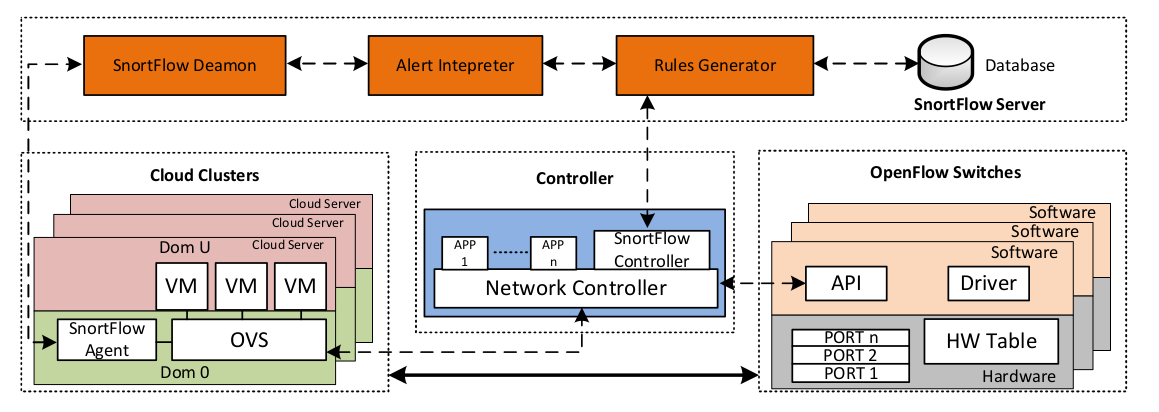
\includegraphics[height=5.5cm]{./pics/snortflow.png}
	\caption{Schéma fonctionnel de Snortflow [\cite{snortflow}]}
	\label{label-image5}
\end{figure}


\subsubsection{SDNIPS}

SDNIPS \cite{sdnips} est une solution reprenant tous les concepts de \textit{SnortFlow} en tentant de répondre à certains paramètres non présents, d'après les auteurs de SDNIPS, dans \textit{SnortFlow}  tels que : l'établissement d'un IDS efficace basé sur SDN et d'une architecture réseau permettant aux mécanismes défensifs des IDS/IPS d'être plus efficace. En effet, le fonctionnement de \textit{SnortFlow} est repris, ainsi que la majorité des composants utilisés (\textit{OpenFlow}, \textit{XenServer}), comme on peut le constater sur la figure \ref{label-image9}.

\begin{figure}[h]
	\center
	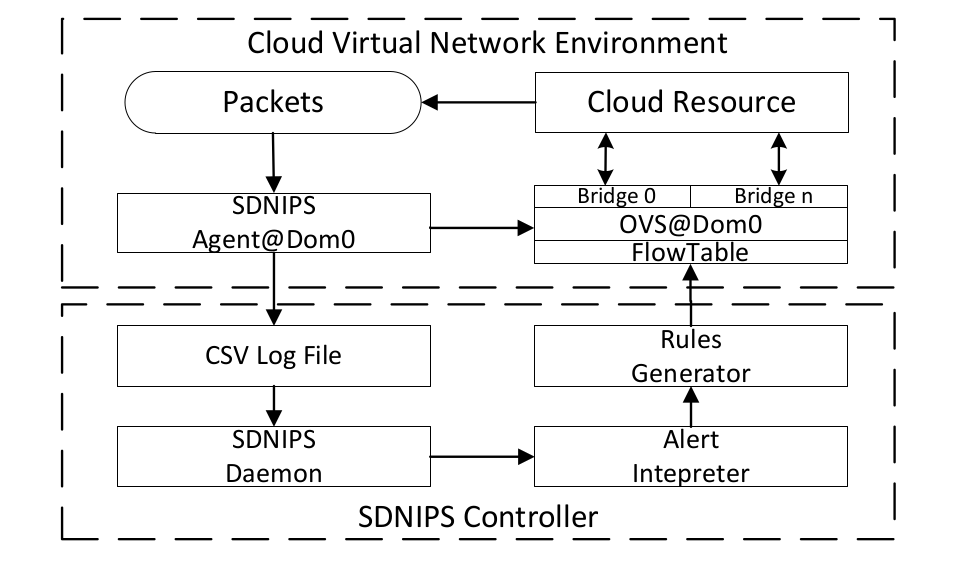
\includegraphics[height=5.5cm]{./pics/SDNIPS_fonctionnement.png}
	\caption{Fonctionnement de SDNIPS \cite{sdnips}}
	\label{label-image9}
\end{figure}

La principale différence entre les deux NIDS se traduit par une différence d'architecture. La figure \ref{label-image6} permet de visualiser l'architecture proposée par SDNIPS. \textit{Open vSwitch} est le \textit{switch} \textit{OpenFlow} et se compose de deux éléments dans l'espace utilisateur : \textit{ovsdb-server} et \textit{ovs-switchd}. Une des principales différences proposées est le déploiement direct de \textit{Snort} dans Dom0. Dom0 permet la détection et le traitement des paquets. En injectant \textit{Snort} dans Dom0, la détection des chemins virtuels vers les \textit{Virtual Interface} (VIF) s'effectue nativement dans OVS et offre une meilleure performance, car \textit{Snort} analyse et gère tous les réseaux virtuels dans le domaine privilégié.

\begin{figure}[h]
	\center
	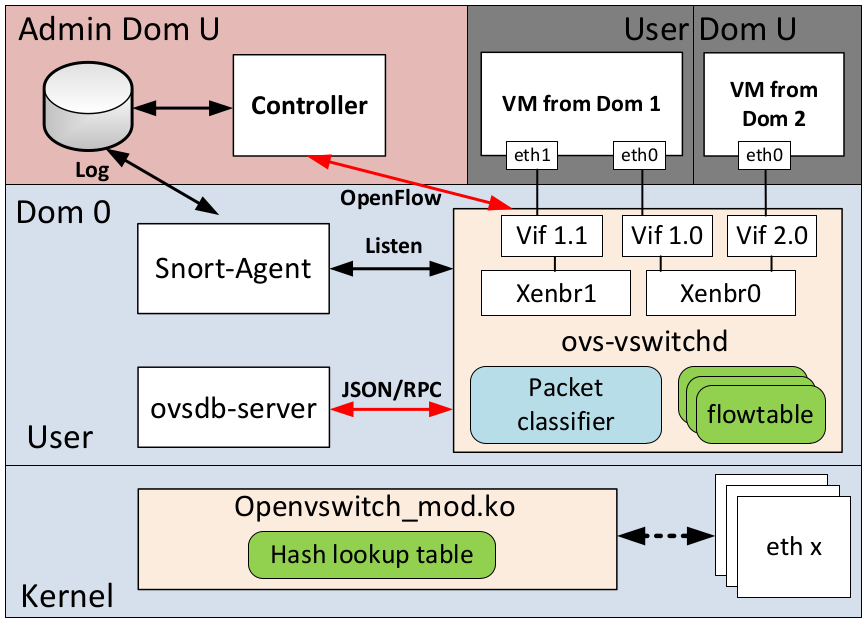
\includegraphics[height=5.5cm]{./pics/SDNIPS_architecture.png}
	\caption{Architecture de SDNIPS \cite{sdnips}}
	\label{label-image6}
\end{figure}


\subsubsection{Comparaison de Snortflow et SDNIPS}

\textit{SnortFlow} et SDNIPS sont tous les deux des systèmes IPS/IDS basés sur SDN générant dynamiquement des contre-mesures contre des attaques sur le réseau. 
Cependant, la faiblesse du papier de \textit{SnortFlow} est son manque d'évaluation et de comparaison. Les comparaisons effectuées n'apportent pas d'informations supplémentaires sur l'efficacité de \textit{SnortFlow}. Au contraire, SDNIPS apporte une comparaison entre le NIDS proposé et l'IPS "traditionnel" (\textit{Snort}/IPTables). Pour cette comparaison, ils ont inondé le réseau d'attaque DoS et ICMP. Il apparaît que SDNIPS détecte tous les paquets malveillants jusqu'à une limite de 15 000 paquets par seconde. L'IPS "traditionnel", lui, ne permet pas de détecter tous les paquets pendant une courte période et les auteurs notent que seuls 13,72\% des paquets ICMP sont détectés comme malveillants. On constate donc une différence importante de performance entre les deux outils. SDNIPS renforce la sécurité du cloud en détectant les anomalies, qu'elles soient nombreuses ou non. Ce type de comparaison est absente du papier présentant \textit{SnortFlow}. En conclusion, les deux papiers présentent des solutions similaires, mais l'absence d'une réelle évaluation de \textit{SnortFlow} justifie la préférence de mettre en avant SDNIPS comme NIDS dans ce rapport.

\begin{figure}[h]
	\center
	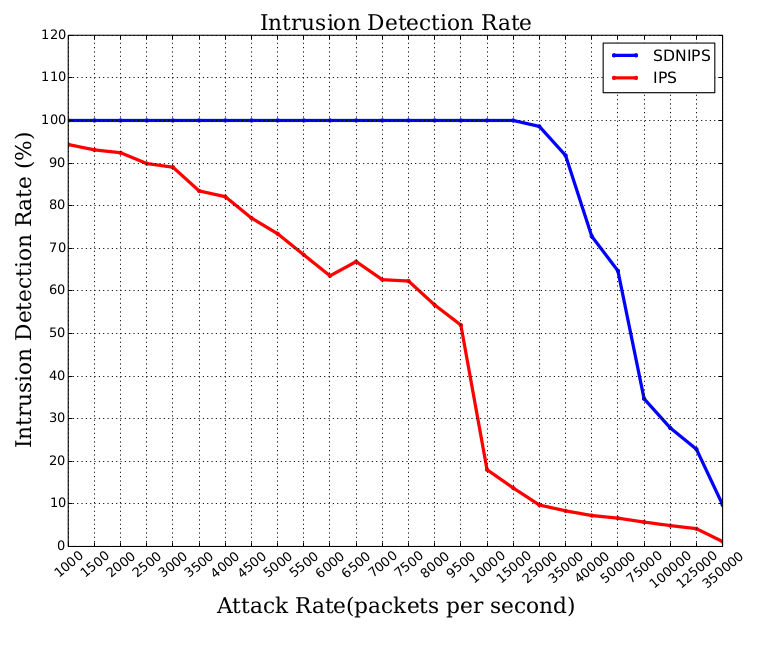
\includegraphics[height=6.5cm, width=10.5cm]{./pics/performance_SDNIPS.png}
	\caption{Évaluation du taux de détection d'intrusion entre un Snort/IPTable et SDNIPS \cite{sdnips}}
	\label{label-image10}
\end{figure}

\subsection{Firewall avec arbre de règle}
Pour conclure sur la sécurité des échanges intra-cloud, on ne pourra pas se passer d'un \textit{firewall}. La solution proposée par Xiangjian He et al. propose un \textit{firewall} sécurisé et performant. Il apparaît différent des \textit{firewalls} traditionnels, car il fonctionne via un arbre de règles et non pas une liste de règles (respectivement, \textit{Tree-rule} et \textit{Listed-rule}). Il propose un arbre et un ensemble de règles hiérarchiques, apparu dans les manuels de \textit{Cisco Services Switch} (CSS). Les \textit{Listed-rule firewall} apparaissent limité, car ce type de \textit{firewall} pose des problèmes de performance, de sécurité, mais également une difficulté à exploiter correctement ce type de \textit{firewall}. Dans ce papier, Xiangjian He et al. nous démontrent les différentes failles d'un \textit{Listed-rule firewall}. En premier lieu, la présence de \textit{shadowed rule} qui est l'une des grandes failles, car c'est une règle qui ne correspond à aucune entrée et pouvant créer ainsi des problèmes de sécurité et de performance. Autre inconvénient, les changement des positions des règles (dans le but d'affecter une règle plutôt qu'une autre pour un paquet) peut engendrer la modification de la politique de sécurité du \textit{firewall} et des failles de sécurité peuvent apparaître. De plus, des règles redondantes sont possibles et peuvent impacter la performance d'un \textit{firewall}. Un autre point négatif est la configuration d'un \textit{Listed-rule firewall}. En effet, un administrateur réseau a le devoir de localiser les plus grosses adresses réseaux aux plus petites (\textit{difficult to use}). Et enfin, les recherches séquentielles (ici recherche séquentielle des règles) pose des problèmes de rapidité et de performance.

La figure \ref{label-image7} permet de visualiser la forme du \textit{firewall} présenté dans le papier de Xiangjian He et al. Le \textit{firewall} lit les données contenues dans l'en-tête des paquets et va comparer les informations du paquet avec les règles des différents nœuds. On peut constater, sur la figure \ref{label-image7}, que à chaque nœud, des attributs différents sont comparés (Destination IP, Destination Port, Source IP). On peut donc spécifier une action spécifique pour certains paquets ou certains utilisateurs. De plus, les attributs présentés sont des exemples, on peut également travailler avec d'autres attributs ou bien même interchanger la place des différents attributs, c'est-à-dire placer la \textit{Destination Port} dans le premier nœud et la \textit{Destination IP} dans le deuxième nœud. Ce \textit{Tree-rule firewall} résout tous les problèmes posés par un \textit{Listed-rule firewall}. En effet, le \textit{firewall} proposé ne pose plus de problèmes de sécurité : les utilisateurs n'ont plus besoin d'effectuer des changements de position des règles et les \textit{shadowed rule} et les règles redondantes n'existent pas dans ce type de \textit{firewall}. Les paquets reçus passent les différents nœuds et suivent un chemin. Si aucun chemin n'est trouvé pour un paquet reçu, c'est-à-dire qu'il ne \textit{match} pas avec une règle contenue dans les nœuds pour un certain attribut, il est alors supprimé(\textit{Deny}). Sinon, on affecte une action spécifique (\textit{Accept}). Ensuite, l'exploitation et la configuration d'un \textit{Tree-rule firewall} est facile, il suffit d'intégrer les différentes informations dans les différentes colonnes des nœuds. Enfin, la complexité d'un arbre de règle est bien moins coûteuse qu'une liste de règles. Selon les auteurs, cette comparaison revient à comparer un arbre binaire de recherche et une recherche linéaire. 

\begin{figure}[h]
	\center
	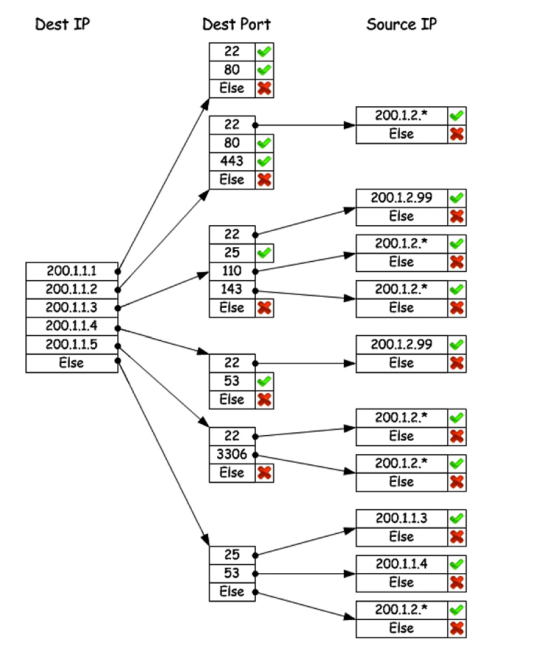
\includegraphics[height=8.5cm,width=11cm]{./pics/tree_rule_firewall.png}
	\caption{Structure d'un \textit{Tree-rule firewall} \cite{tree_rule_firewall}}
	\label{label-image7}
\end{figure}

De plus, IPTables apporte la plupart des fonctionnalités de base d'un \textit{firewall} (filtrage dynamique, translation de port et d'adresse, filtrage au niveau 2), mais lorsque le nombre de règles commence à être très grand, IPTables n'est plus capable d'apporter des performances satisfaisantes : moins de la moitié des règles sont atteintes avec IPTables quand le nombre de règles est de 5000. De plus, le CPU approche les 100\% d'utilisation. \textit{Tree-rule firewall} apporte toujours une excellente performance, malgré un nombre de règle important. Enfin, le CPU n'atteint même pas les 5\% d'utilisation. On peut donc affirmer que les performances du \textit{Tree-rule firewall} sont largement supérieur à IPTables. 
\newline
Pour conclure sur ce \textit{Tree-rule firewall}, les auteurs proposent  l'utilisation du \textit{firewall} sur un environnement cloud et proposent une comparaison entre différents \textit{firewall}. On constate via la figure \ref{label-image11} que le \textit{Tree-rule firewall} apporte des performances supplémentaires par rapport aux autres \textit{firewall}. La sécurité et les performances apportées par le \textit{Tree-rule firewall} sont importantes et vérifiées par les différentes comparaisons effectuées dans ce papier.

\begin{figure}[h]
	\center
	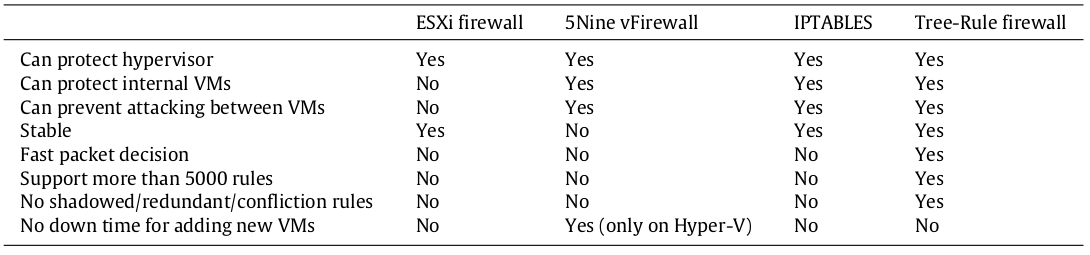
\includegraphics[height=3.5cm,width=15cm]{./pics/comparatif_firewall.png}
	\caption{Comparaison des fonctionnalités de différents\textit{firewall} dans un environnement cloud \cite{tree_rule_firewall}}
	\label{label-image11}
\end{figure}


	\begingroup
\renewcommand{\cleardoublepage}{}
\renewcommand{\clearpage}{}
\chapter{Conclusion}
\endgroup

Le but de ce chapitre est de résumer les contributions de ce Travail
d'Étude et de Recherche, à savoir une classification des différentes catégories
de problèmes de sécurité dans le cloud informatique, une étude des différentes
solutions de la littérature, et une analyse des points qui pourraient être
améliorés.
La section~\ref{sec:con} résume les différentes contributions de ce document,
et la section~\ref{sec:per} énumère les potentielles contributions futures,
comme par exemple les points faibles des architectures actuelles.

\section{Contributions}\label{sec:con}

Dans ce sujet du Travail d'Étude et de Recherche, nous nous sommes intéressés à la sécurité de systèmes de \textit{workflow}. Nous nous sommes limités à un cas d'étude particulier : le cloud computing. Pour sécuriser ce système, il est nécessaire d'établir la surveillance globale du trafic, afin de détecter l’ensemble des attaques perpétrées, y compris les attaques internes à la structure. Les solutions de sécurité traditionnelles
réalisent généralement leurs analyses en ne considérant que le trafic qui transite localement.
De même, les traitements réalisés par ces équipements estiment que les attaques proviennent exclusivement de l’extérieur du réseau. Cette vision n’est malheureusement plus applicable pour
des réseaux comme le cloud, où un utilisateur malicieux peut facilement obtenir des ressources puissantes, et à bas coût, pour réaliser des attaques provenant du réseau interne. Cependant, le cloud ne pose pas que des problèmes de sécurité au niveau du réseau. Le stockage et la virtualisation posent également de nouveaux problèmes de sécurité.

Pour palier à ces problèmes, ce document propose différentes pistes à établir dans un cloud dans le but d'améliorer la sécurité du réseau principalement, mais également au niveau de la virtualisation et du stockage. Tout d'abord, nous avons proposé deux solutions différentes pour améliorer le stockage dans le cloud : FADE et SecCloud. Ensuite, nous avons évoqué différentes pistes pour sécuriser la virtualisation et permettre son fonctionnement. Par la suite, une solution a été proposée pour permettre une authentification sécurisée et un contrôle d'accès efficace. Puis, nous nous sommes intéressés au réseau, plus précisément aux communications inter-cloud et intra-cloud. Une architecture DMVPN (\textit{Dynamic Multipoint VPN}) garantit l'utilisation d'IPSecVPN et résout les différents problèmes posés par les architectures inter-cloud actuelles. La partie intra-cloud se compose par l'utilisation d'un NIDS et d'un \textit{firewall}. Deux NIDS sont proposés, SnortFlow et SDNIPS. Cependant, seul SDNIPS propose une véritable application et différentes comparaisons prouvant l'efficacité du NIDS dans un environnement cloud. Enfin, le  \textit{Tree-rule firewall} est mis en avant. Ce dernier se différencie des \textit{firewalls} classiques, appelés \textit{Listed-rule firewall}, car il résout tous les problèmes de performance et de sécurité associés aux \textit{Listed-rule firewall}.

\section{Perspectives}\label{sec:per}

Tout d'abord, les premières perspectives envisagées par ce document sont l'établissement et l'intégration des pistes étudiées dans un environnement cloud, plus précisément dans un cloud public. De plus, les différents pistes abordées présentent également des défauts et peuvent faire l'objet d'évolutions. Par exemple, le \textit{Tree-rule firewall} ne traite pas encore IPv6, NAT (\textit{Network Address Translation}) ou encore les VPN. Si l'intégration du VPN s'effectue, il peut paraître très pertinent d'associer l'architecture inter-cloud proposée avec des règles de \textit{firewall}. 

Malheureusement, le cloud évolue sur plusieurs nouvelles couches réseaux et des nouvelles technologies continuent d'apparaître et d'évoluer à une vitesse vertigineuse. Il existe un vrai décalage entre la sécurité et les technologies actuelles ce qui implique un décalage entre les menaces actuelles de sécurité et les solutions et le périmètre de sécurité établis.


	\begingroup
    \renewcommand{\cleardoublepage}{}
    \renewcommand{\clearpage}{}
	\printglossaries
    \endgroup

	\begingroup
    \renewcommand{\cleardoublepage}{}
    \renewcommand{\clearpage}{}
	\bibliography{\jobname}
	\bibliographystyle{plain}
    \endgroup

\end{document}
